\section{Experimentos}

%Normal Slide (copy, paste and modify this slide for longer presentations)
\begin{frame}
\frametitle{\secname} %Title
\framesubtitle{Comparativa de los experimentos} %Subtitle
\rmfamily %Font
\color{black} %Color
\begin{table}
    \centering
    \resizebox{0.75\textwidth}{!}{
    \begin{tabular}{ccccc}
        \toprule
        \texttt{time} & \texttt{TSrock} & \texttt{TSrasp} & \texttt{offset} & \texttt{device} \\
        \midrule
        292 & 119238112796030 & 104592709716803 & -14645403079227 & 192.168.1.111 \\
        1001191222 & 119239113986960 & 104593710167425 & -14645403819535 & 192.168.1.111 \\
        2001485862 & 119240114281600 & 104594710453699 & -14645403827901 & 192.168.1.111 \\
        \vdots & \vdots & \vdots & \vdots & \vdots \\
        \bottomrule
    \end{tabular}
    }
    \caption{Ejemplo de los datos obtenidos de cada dispositivo}
    \label{tab:trace_example}
\end{table}
\vspace{-1.3cm}
\setcounter{subfigure}{0}
\begin{figure}
    \centering
    \subfloat[Desviación acumulada muestra secuencial]{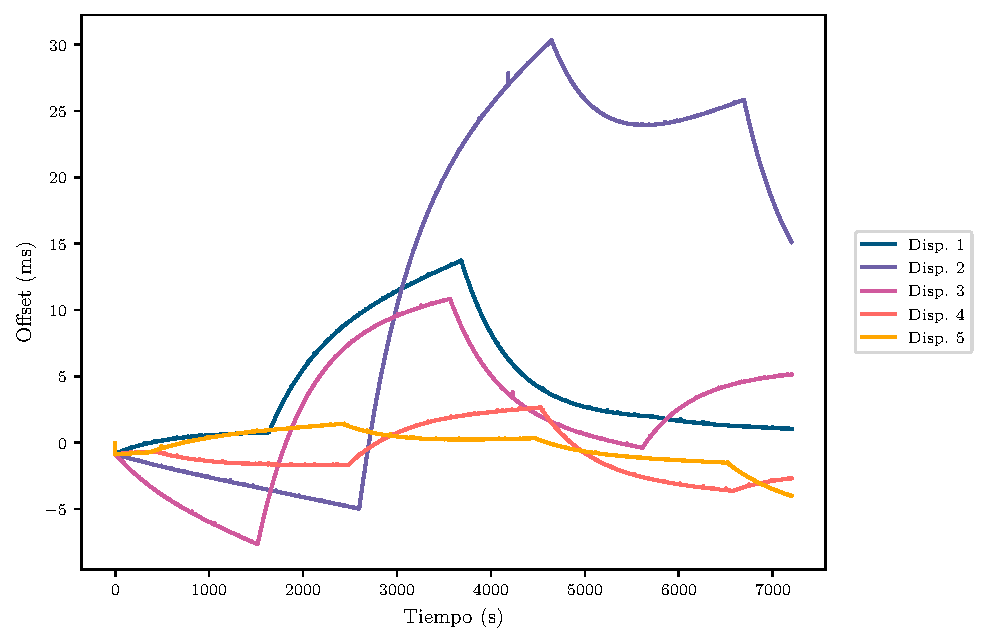
\includegraphics[width=0.5\textwidth]{../Python/plots/individual/offset_plot.pdf}}
    \subfloat[Desviación acumulada muestra paralela]{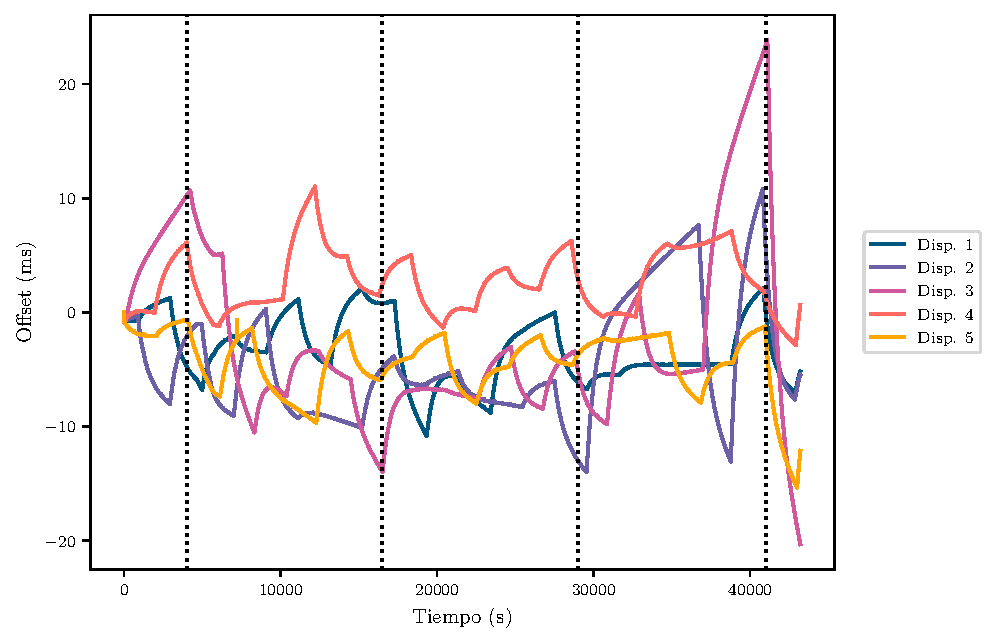
\includegraphics[width=0.5\textwidth]{../Python/plots/parallel/offset_plot.pdf}}
\end{figure}
\end{frame}

%Normal Slide (copy, paste and modify this slide for longer presentations)
\begin{frame}
\frametitle{\secname} %Title
\framesubtitle{Comparativa de los experimentos} %Subtitle
\rmfamily %Font
\color{black} %Color
\setcounter{subfigure}{0}
\begin{figure}
    \centering
    \subfloat[Desviación muestra secuencial]{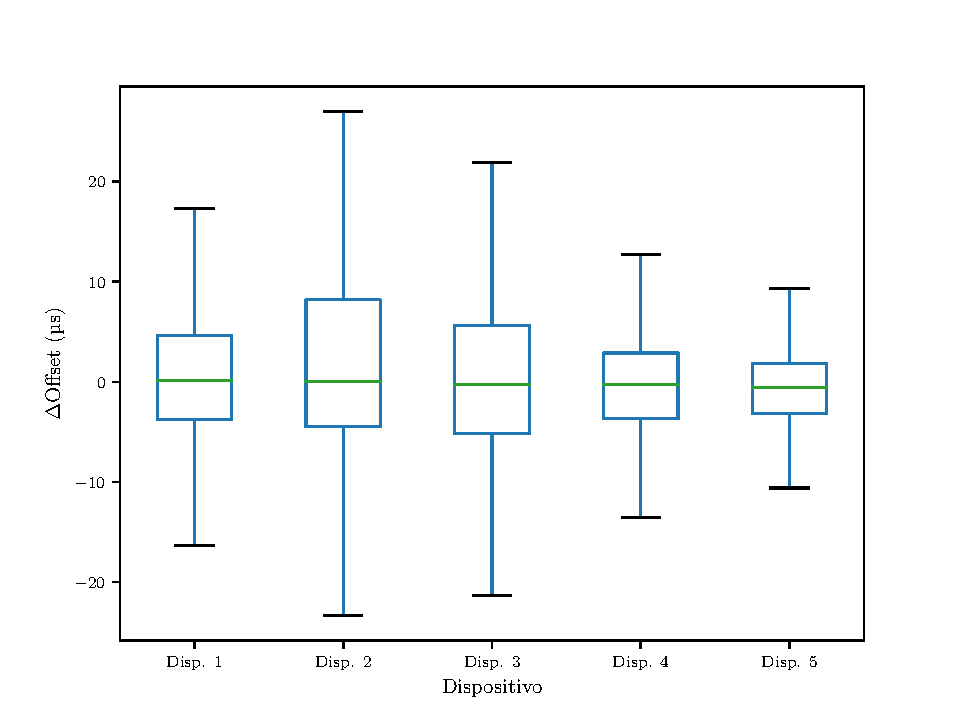
\includegraphics[width=0.5\textwidth]{../Python/plots/individual/boxplot_no_out.pdf}}
    \subfloat[Desviación muestra paralela]{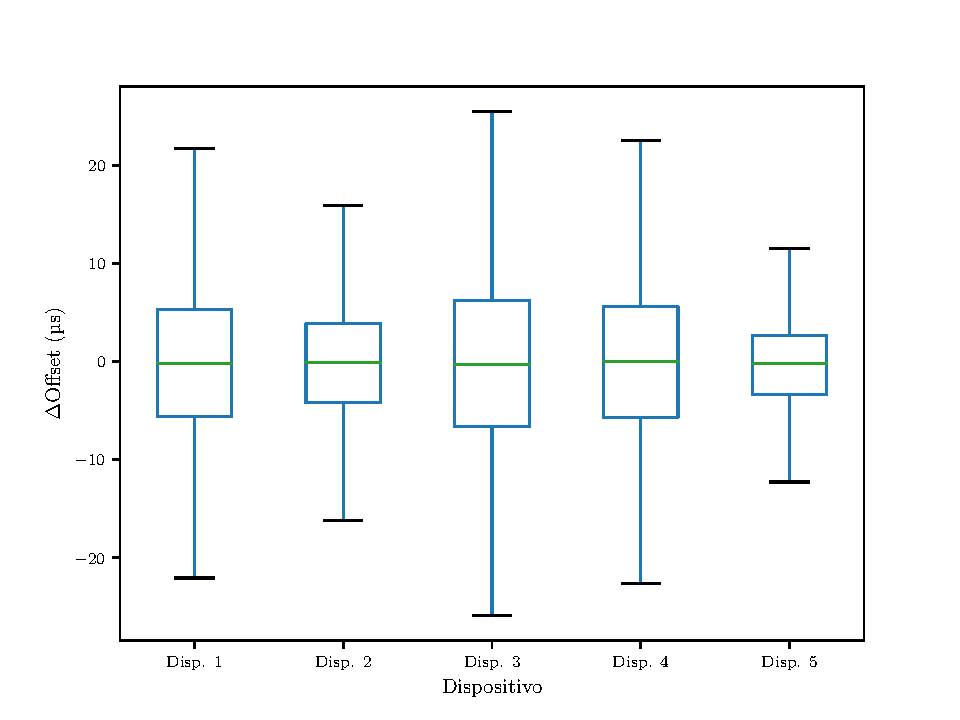
\includegraphics[width=0.5\textwidth]{../Python/plots/parallel/boxplot_no_out.pdf}}
\end{figure}
\end{frame}

%Normal Slide (copy, paste and modify this slide for longer presentations)
\begin{frame}
\frametitle{\secname} %Title
\framesubtitle{Generación de estadísticas y reducción de la \\[-2pt] dimensionalidad} %Subtitle
\rmfamily %Font
\color{black} %Color
\begin{table}
    \centering
    \resizebox{\textwidth}{!}{
        \begin{tabular}{cccccccccccc}
            \toprule
             & Sum & Mean & Median & Mode & Std & IQR & Kurtosis & Skew & Max & Min & Device \\
            \midrule
            1 & -284.0 & -4.733333333333333 & -203.0 & -10750.0 & 6531.321744049499 & 8739.5 & -0.8026364427898236 & 0.266444555013173 & 12077.0 & -10750.0 & Disp. 1 \\
            2 & -65895.0 & -1098.25 & 106.5 & -13344.0 & 3926.559099283938 & 2519.75 & 1.4605213340303709 & -1.1040127142547507 & 7616.0 & -13344.0 & Disp. 2 \\
            3 & 96179.0 & 1602.9833333333333 & 815.0 & -8136.0 & 5010.092595279735 & 6575.5 & -0.39715065367509084 & 0.2484646585713819 & 12831.0 & -8136.0 & Disp. 3 \\
            4 & 109162.0 & 1819.3666666666666 & 2016.5 & -10485.0 & 6159.084454763058 & 8290.5 & -0.7264084617343212 & -0.3858981208999922 & 11469.0 & -10485.0 & Disp. 4 \\
            5 & -81317.0 & -1355.2833333333333 & -2127.0 & -6378.0 & 3665.051390911538 & 2616.5 & 2.701193448053943 & 1.7089231615691112 & 10383.0 & -6378.0 & Disp. 5 \\
            6 & 19928.0 & 332.1333333333333 & -147.0 & -10750.0 & 6613.483928825726 & 10212.0 &     -0.8404647945245984 & 0.23473423365399895 & 12077.0 & -10750.0 & Disp. 1 \\
            \vdots & \vdots & \vdots & \vdots & \vdots & \vdots & \vdots & \vdots & \vdots & \vdots & \vdots & \vdots \\
            \bottomrule
        \end{tabular}
    }
    \caption{Datos estadísticos muestra paralela}
    \label{tab:stats_par}
\end{table}
\vspace{-1cm}
\begin{figure}
    \centering
    \subfloat{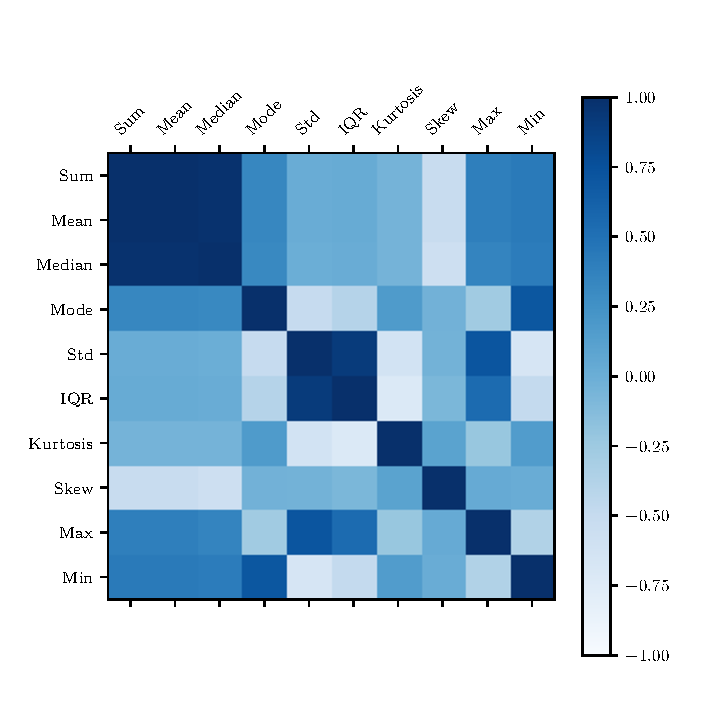
\includegraphics[scale=0.3]{../Python/plots/parallel/correlacion_stats.pdf}}
    \subfloat{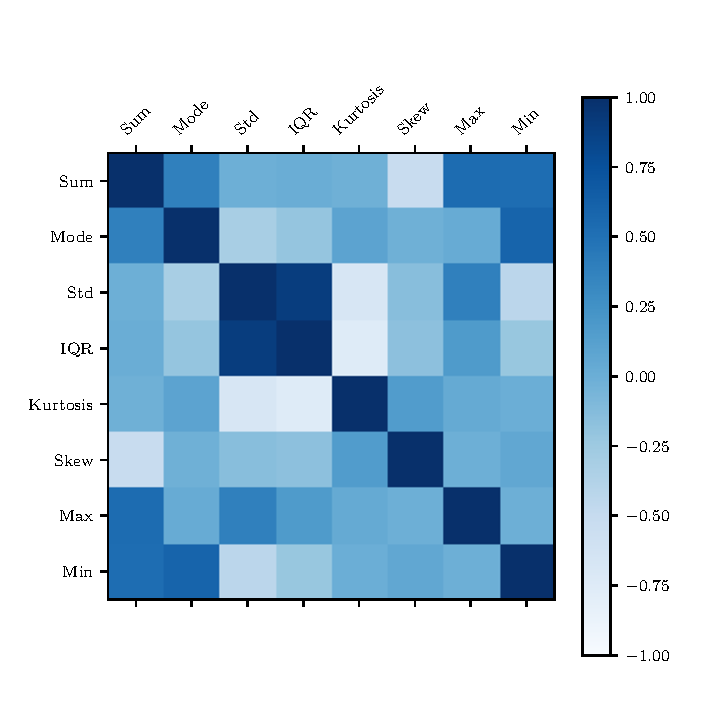
\includegraphics[scale=0.3]{../Python/plots/parallel/correlacion_stats_ftred.pdf}}
    \caption{Correlación entre las variables estadísticas}
    \label{fig:corr}
\end{figure} 
\end{frame}

%Normal Slide (copy, paste and modify this slide for longer presentations)
\begin{frame}
\frametitle{\secname} %Title
\framesubtitle{Particionamiento de los datos} %Subtitle
\rmfamily %Font
\color{black} %Color
\begin{figure}
    \centering
    \hspace{-0.65cm}
    \subfloat[Particionamiento para clasificadores]{
        \resizebox{0.6\textwidth}{!}{
            \begin{tikzpicture}[show background rectangle,background rectangle/.style={fill=white, draw, rounded corners, thick}]
                \node[database,label=below:Datos del dispositivo,database radius=1cm,database segment height=0.5cm] (data) {};
                \node (aux) [right = of data] {};
                \node[database,label=below:Entrenamiento,database radius=0.75cm,database segment height=0.375cm] (train) [above right = 2cm of aux] {};
                \node[database,label=below:Test,database radius=0.75cm,database segment height=0.375cm] (test) [below right = 2cm of aux] {};
                \node[database,label=below:{$\underset{\text{Reducido}}{\text{Entrenamiento}}$},database radius=0.5cm,database segment height=0.25cm] (train2) [right = 3cm of train] {};
                \node (aux2) [right = of train2] {};
                \node[database,label=below:Entrenamiento,label=right:70\%,database radius=0.5cm,database segment height=0.25cm] (train3) [above right = of aux2] {};
                \node[database,label=below:Validación,label=right:30\%,database radius=0.5cm,database segment height=0.25cm] (test) [below right = of aux2] {};
                \draw[-] (1.2,0) -- (aux.center);
                \draw[-] (aux.center) |- (3.4, 2.4) node [above, pos=0.75] {70\%};
                \draw[-] (aux.center) |- (3.4, -2.45) node [below, pos=0.75] {30\%};
                \draw[-] (5.5, 2.4) -- (8, 2.4) node [midway, above] {35\%};
                \draw[-] (9.5, 2.4) -- (aux2.center);
                \draw[-] (aux2.center) |- (11.3, 4.1);
                \draw[-] (aux2.center) |- (11.3, 0.66);
            \end{tikzpicture}
        }
    }
    \subfloat[Particionamiento para la detección de anomalías]{
        \resizebox{0.4\textwidth}{!}{
            \begin{tikzpicture}[show background rectangle,background rectangle/.style={fill=white, draw, rounded corners, thick}]
                \node[database,label=below:Datos,database radius=1cm,database segment height=0.5cm, outer sep=0.5cm] (data) {};
                \node[database,label=below:$\underset{\text{Disp. }x}{\text{Datos}}$,database radius=0.75cm,database segment height=0.375cm, outer sep=0.3cm] (disp_data) [above right = 0cm and 2cm of data] {};
                \node[database,label=below:$\underset{\text{sin Disp. }x}{\text{Datos}}$,database radius=0.75cm,database segment height=0.375cm, outer sep=0.3cm] (disp_out_data) [below right = 0cm and 2cm of data] {};
                
                \node[database,label=below:Entrenamiento,database radius=0.75cm,database segment height=0.375cm, outer sep=0.3cm] (train) [above right = -0.5cm and 2cm of disp_data] {};
                \node[database,label=below:Test,database radius=0.75cm,database segment height=0.375cm, outer sep=0.3cm] (test) [below right = -1cm and 2cm of disp_data] {};
                
                
                \node (train2) [above right = -1cm and 2cm of disp_out_data] {\Huge\phantom{---}\xmark};
                \node[database,label=below:Test,database radius=0.75cm,database segment height=0.375cm, outer sep=0.3cm] (test2) [below right = -1cm and 2cm of disp_out_data] {};
                
                \draw[-] (data) -| (2.4,0) |- (disp_data);
                \draw[-] (data) -| (2.4,0) |- (disp_out_data);
                
                \draw[-] (disp_data) -| (6.4, 4) |- (train) node [above, pos=0.75] {80\%};
                \draw[-] (disp_data) -| (6.4, 4) |- (test) node [above, pos=0.75] {20\%};
                
                \draw[-] (disp_out_data) -| (6.4, -4) |- (train2) node [above, pos=0.75] {80\%};
                \draw[-] (disp_out_data) -| (6.4, -4) |- (test2) node [above, pos=0.75] {20\%};
                
            \end{tikzpicture}
        }
    }
\end{figure}
\end{frame}

\section{Resultados}

%Normal Slide (copy, paste and modify this slide for longer presentations)
\begin{frame}
\frametitle{\secname} %Title
\framesubtitle{Comparativa de algoritmos} %Subtitle
\rmfamily %Font
\color{black} %Color
\begin{figure}
    \centering
    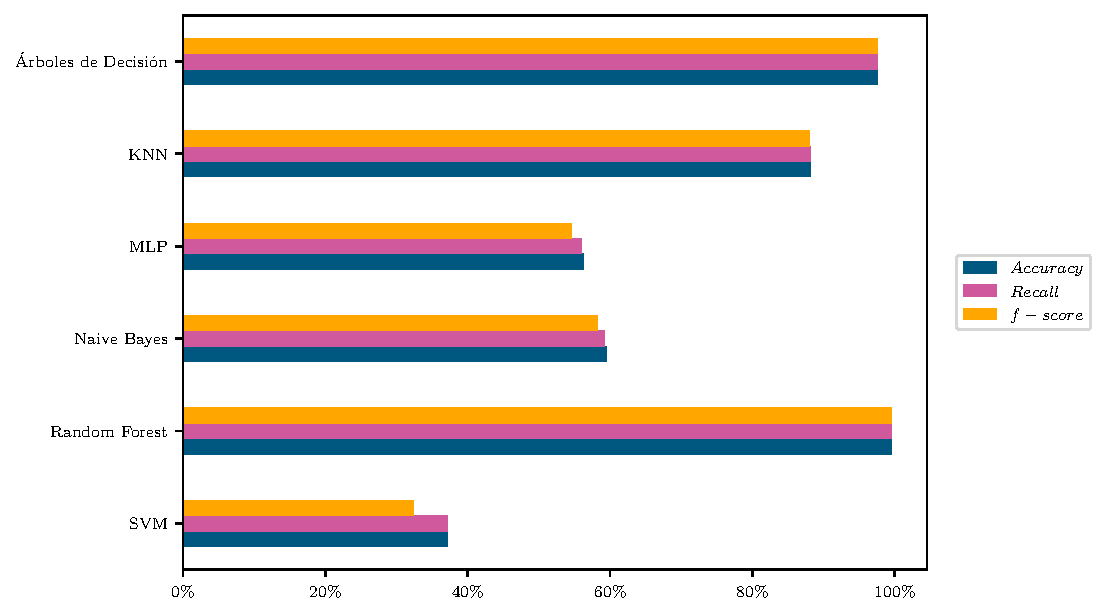
\includegraphics[width=0.6\textwidth]{../Python/plots/parallel/model_results.pdf}
    \caption{Algoritmos de clasificación}
\end{figure} 
\vspace{-1cm}
\begin{table}
    \centering
    \resizebox{0.5\textwidth}{!}{
        \begin{tabular}{lcccccc}
    \toprule
     & \multicolumn{2}{c}{\texttt{Isolation Forest}} & \multicolumn{2}{c}{\texttt{Local Outlier Factor}} & \multicolumn{2}{c}{\texttt{OneClass-SVM}} \\
    \cmidrule(lr){2-3}\cmidrule(lr){4-5}\cmidrule(lr){6-7}
    & $Recall$ & $TNR$ & $Recall$ & $TNR$ & $Recall$ & $TNR$ \\
    \midrule
     Disp. 1 & 95.12\% & 10.36\% & 98.99\% & 10.68\% & 49.48\% & 58.24\% \\
     Disp. 2 & 94.98\% & 28.87\% & 98.45\% & 57.74\% & 50.90\% & 70.36\% \\
     Disp. 3 & 94.80\% & 13.90\% & 98.73\% & 13.64\% & 49.84\% & 52.65\% \\
     Disp. 4 & 95.80\% & 16.61\% & 98.88\% & 8.74\% & 50.54\% & 64.66\% \\
     Disp. 5 & 94.89\% & 46.99\% & 98.63\% & 77.98\% & 49.53\% & 94.59\% \\
    \bottomrule
\end{tabular}

    }
    \caption{Algoritmos de detección de anomalías}
\end{table}
\end{frame}


%Normal Slide (copy, paste and modify this slide for longer presentations)
\begin{frame}
\frametitle{\secname} %Title
\framesubtitle{Resultados finales} %Subtitle
\rmfamily %Font
\color{black} %Color
\begin{minipage}{0.4\textwidth}
Resultados:
    \begin{itemize}
        \item Accuracy: 99.38\%
        \item $f$-score: 99.38\%
        \item Recall: 99.39\%
    \end{itemize}
\end{minipage}
\begin{minipage}{0.43\textwidth}
\begin{figure}
    \centering
    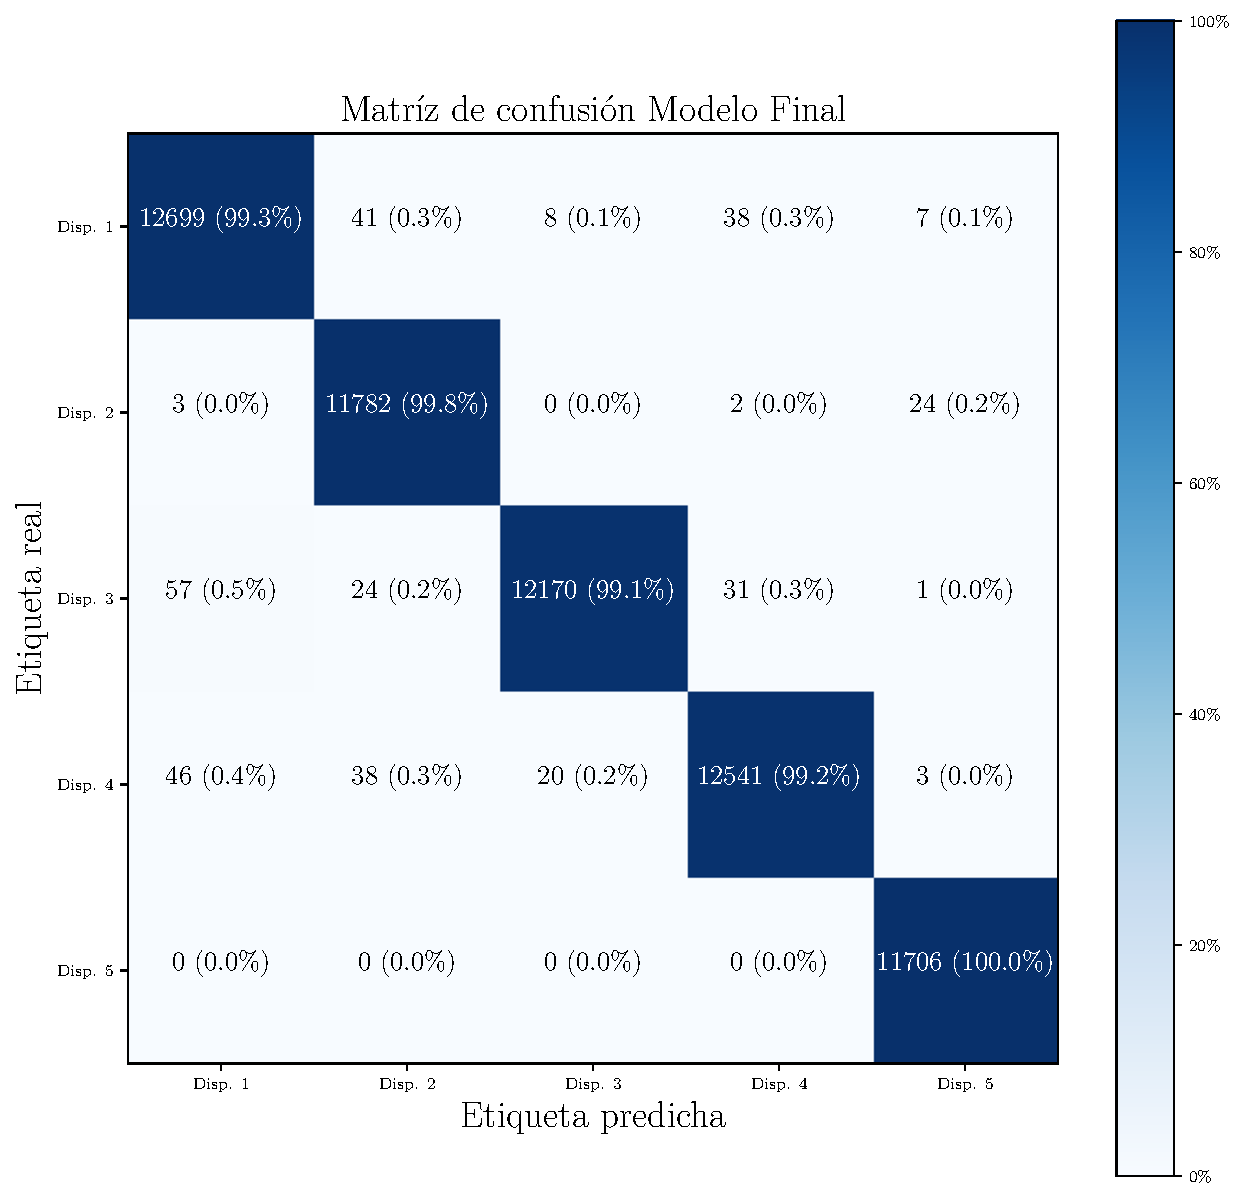
\includegraphics[width=1.6\textwidth]{../Python/plots/parallel/final_model_matrix.pdf}
\end{figure}
\end{minipage}
\end{frame}

